\def\probtitle{피보나치 기념품}
\def\probno{F} % 문제 번호

\begin{problem}{\probno{}. \probtitle{}}

\begin{center}
    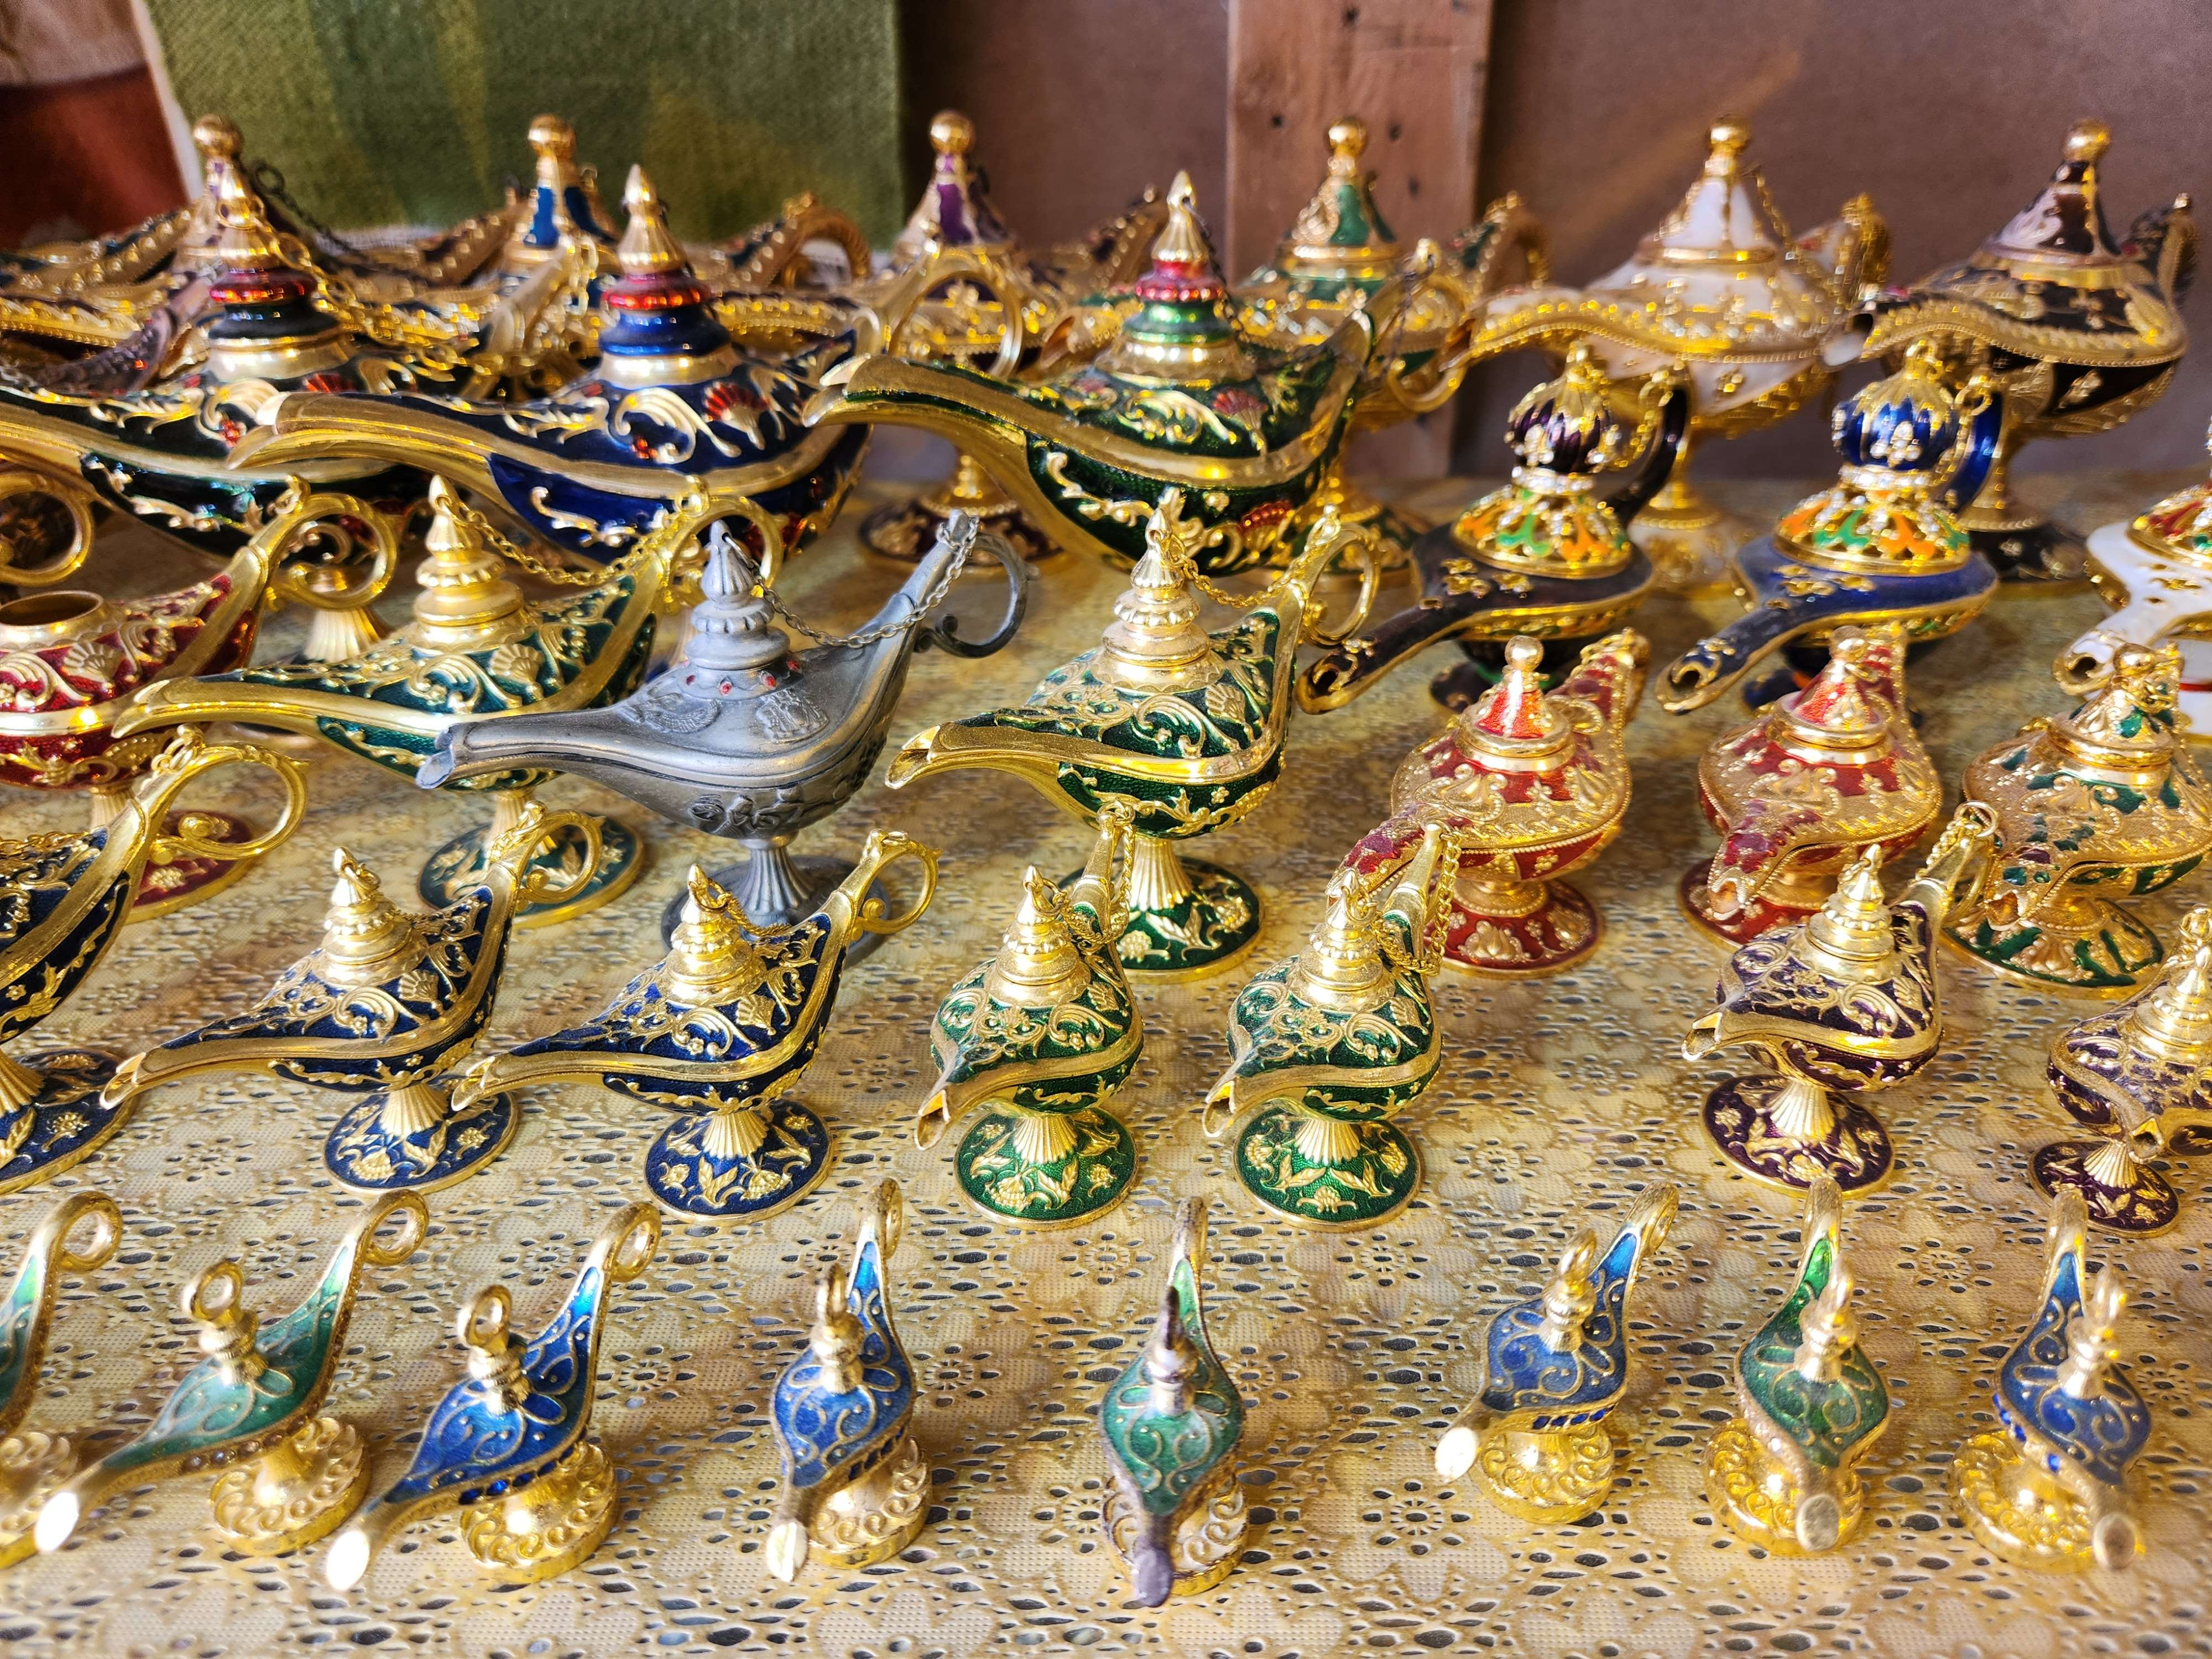
\includegraphics[width=0.65\linewidth]{2024/fibonacci-partition/image/lamp.jpg}
\end{center}

피보나치 수열은 다음과 같이 정의되는 수열이다.

\begin{itemize}[topsep=0pt,noitemsep]
    \item $F_1 = 1$
    \item $F_2 = 1$
    \item $F_n = F_{n-1} + F_{n-2}$ (단, $n \ge 3$)
\end{itemize}

정휘는 이집트 룩소르의 한 시장에서 피보나치 수가 적혀 있는 $N$개의 기념품을 구매했다. $x (1 \le x \le N)$번 기념품에는 $F_x$가 적혀 있다.

정휘는 피보나치 수열을 좋아하는 세림이와 성주에게 기념품을 선물하려고 한다. 하지만 한 명에게 너무 많은 기념품을 주면 기념품을 적게 받은 사람이 슬퍼할 수 있기 때문에, 두 명이 받게 될 \textbf{기념품에 적힌 피보나치 수의 합}이 같아지도록 선물을 분배하려고 한다. 구매한 기념품의 개수 $N$에 따라 $N$개의 기념품을 전부 나눠주지 못할 수 있는데, 이때는 최대한 \textbf{많은 개수}의 기념품을 나눠주려고 한다.

나눠주는 기념품의 개수를 최대화하면서, 두 명이 받는 기념품에 적힌 수의 합이 같도록 기념품을 나눠주는 방법을 구해보자. 두 사람에게 1개 이상의 기념품을 나눠주는 방법은 항상 존재한다.

\InputFile

첫째 줄에 정휘가 구매한 기념품의 개수 $N$이 주어진다.

\OutputFile

첫째 줄에 세림이가 받을 기념품의 개수 $X$를 출력한다.

둘째 줄에 세림이가 받을 기념품들의 번호 $A_1, A_2, \cdots, A_X$를 공백으로 구분해서 출력한다.

셋째 줄에 성주가 받을 기념품의 개수 $Y$를 출력한다.

넷째 줄에 성주가 받을 기념품들의 번호 $B_1, B_2, \cdots, B_Y$를 공백으로 구분해서 출력한다.

가능한 분배 방법이 여러 가지면 그중 아무거나 하나만 출력하라.

\pagebreak

\Constraints

\begin{itemize}[topsep=0pt,noitemsep]
    \item $2 \leq N \leq 2\,000$
    \item $X, Y \ge 1$
    \item $1 \le A_i \le N (1 \le i \le X)$
    \item $1 \le B_j \le N (1 \le j \le Y)$
    \item $A_1, A_2, \cdots, A_X, B_1, B_2, \cdots, B_Y$는 서로 다른 수이다.
    \item 입력으로 주어지는 수는 모두 정수이다.
\end{itemize}

\Example

\begin{example}
    \exmpfile{./example/01.in.txt}{./example/01.out.txt}%
    \exmpfile{./example/02.in.txt}{./example/02.out.txt}%
\end{example}

\end{problem}